\chapter{Obtención de la región de interés}
\label{cha:Obtención de la región de interés}

\begin{FraseCelebre}
  \begin{Frase}
    Texto.
  \end{Frase}
  \begin{Fuente}
    Autor texto
  \end{Fuente}
\end{FraseCelebre}

\section{Proyección de píxeles en la cámara a coordenadas 3D}
\label{sec:Proyección de píxeles en la cámara a coordenadas 3D}

\begin{center}
$P = P2 * R_0\_rect * Tr\_velo\_to\_cam$
\end{center}

\begin{center}
$
P * (inv(Tr\_velo\_to\_cam) * inv(R_0\_rect) * inv(P2)) =
\begin{bmatrix}
1.00000e^{+00} & -3.64291e^{-17} & 1.13686e^{-13} \\
-6.93889e^{-17} & 1.00000e^{+00} & -8.88178e^{-14} \\
-3.38813e^{-21} & 8.90893e^{-19} & 1.00000e^{+00} \\
\end{bmatrix}
$
\end{center}

\begin{center}
$
P * (inv(P2 * R_0\_rect * Tr\_velo\_to\_cam)) =
\begin{bmatrix}
1.00000e^{+00} & 1.25767e^{-16} & 1.13686e^{-13} \\
1.04083e^{-16} & 1.00000e^{+00} & -1.42108e^{-13} \\
7.52165e^{-19} & -6.06475e^{-19} & 1.00000e^{+00} \\
\end{bmatrix}
$
\end{center}

\begin{center}
$
\begin{bmatrix}
wx_{1i}\\wy_{1i}\\w
\end{bmatrix}
= P_2
\begin{bmatrix}
x_{1c}\\y_{1c}\\z_{1c}\\1
\end{bmatrix} = 
\begin{bmatrix}
f&0&u_0&t_x\\0&f&v_0&t_y\\0&0&1&t_z
\end{bmatrix}
\begin{bmatrix}
x_{1c}\\y_{1c}\\z_{1c}\\1
\end{bmatrix}
$
\end{center}

\begin{center}
$
\begin{bmatrix}
x_{1l}\\y_{1l}\\z_{1l}\\1
\end{bmatrix}
= T_{v2c}^{-1} * R_0^{-1} *
\begin{bmatrix}
x_{1c}\\y_{1c}\\z_{1c}\\1
\end{bmatrix}
$
\end{center}

\begin{center}
$wx_{1i} = f x_{1c} + u_0 z_{1c} + t_x$\\
$wy_{1i} = f y_{1c} + v_0 z_{1c} + t_y$\\
$w = z_{1c} + t_z$\\
$d = \sqrt{x_{1c}^2 + y_{1c}^2 + z_{1c}^2}$
\end{center}

\begin{center}
$f = 707.0493$\\
$u_0 = 604.0814$\\
$v_0 = 180.5066$\\
$t_x = 45.75831$\\
$t_y = -0.3454157$\\
$t_z = 0.004981016$
\end{center}

\begin{center}
$w x_{1i}=707.0493 x_{1c}+604.0814 z_{1c}+45.75831$\\
$w y_{1i} = 707.0493 y_{1c} + 180.5066 z_{1c} + -0.3454157$\\
$w = z_{1c} + 0.004981016$\\
$d = \sqrt{x_{1c}^2 + y_{1c}^2 + z_{1c}^2}$
\end{center}

\section{Obtención del tronco geométrico}
\label{sec:Obtención del tronco geométrico}

Rotación de eje frontal como en Frustum PointNets

\begin{figure}[H]
	\begin{minipage}{0.495\textwidth}
		\centering
		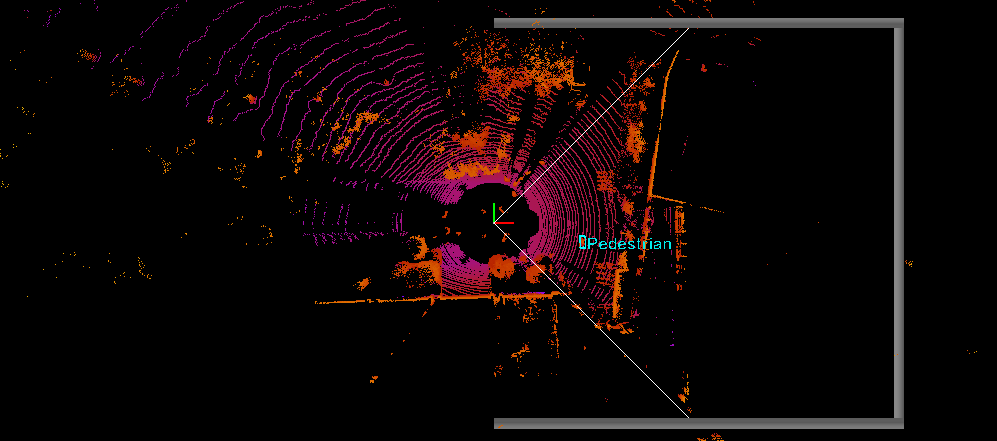
\includegraphics[width=1\linewidth]{Book/figures/7_roi/kitti_pcl_0.png}
	\end{minipage}\hfill
	\begin{minipage}{0.495\textwidth}
		\centering
		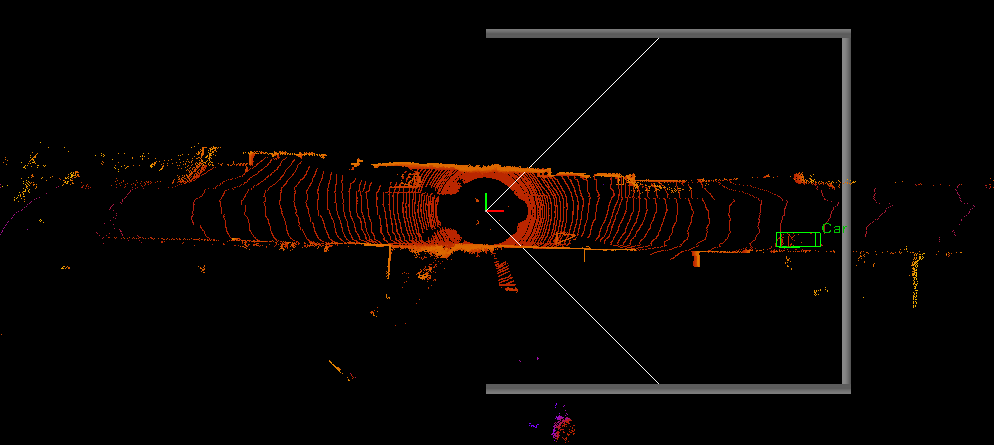
\includegraphics[width=1\linewidth]{Book/figures/7_roi/kitti_pcl_2.png}
	\end{minipage}
	\caption{Nubes de puntos de KITTI con su ground-truth.}
	\label{fig:Nubes de puntos de KITTI con su ground-truth.}
\end{figure}

\begin{figure}[H]
	\begin{minipage}{0.495\textwidth}
		\centering
		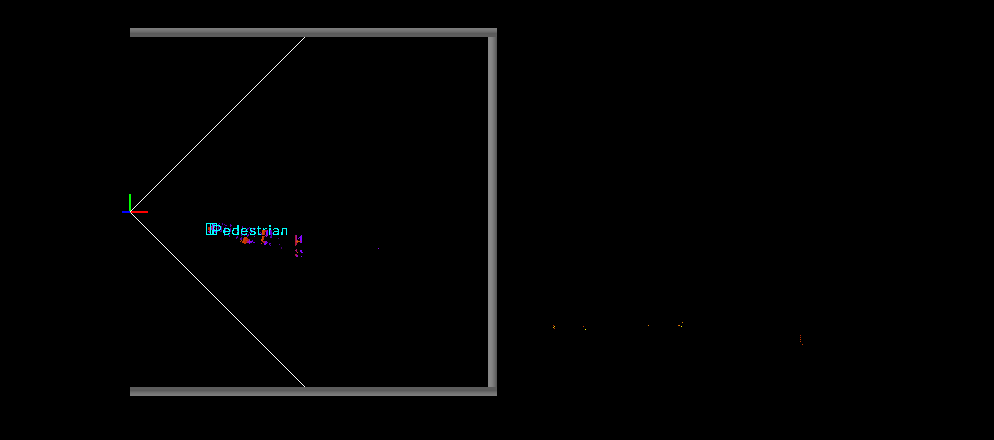
\includegraphics[width=1\linewidth]{Book/figures/7_roi/kitti_pcl_filt_0.png}
	\end{minipage}\hfill
	\begin{minipage}{0.495\textwidth}
		\centering
		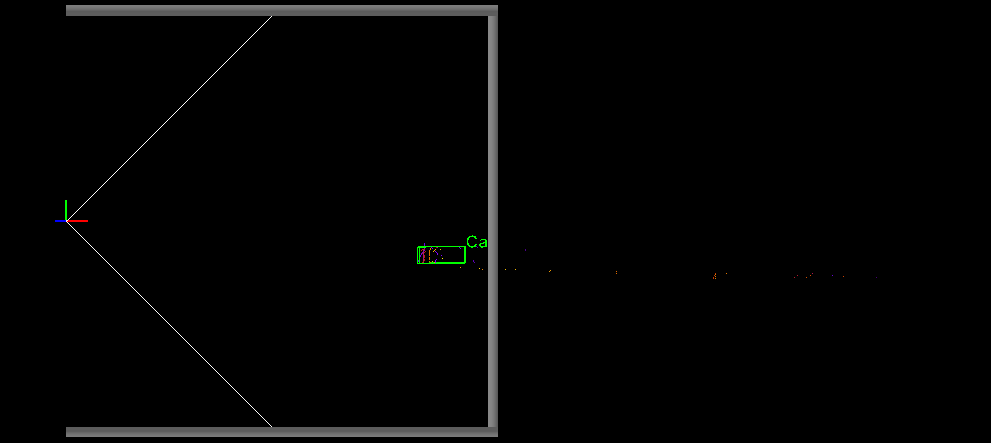
\includegraphics[width=1\linewidth]{Book/figures/7_roi/kitti_pcl_filt_2.png}
	\end{minipage}
	\caption{Nubes de puntos de KITTI filtradas por las detecciones 2D.}
	\label{fig:Nubes de puntos de KITTI filtradas por las detecciones 2D.}
\end{figure}

\begin{figure}[H]
	\begin{minipage}{0.495\textwidth}
		\centering
		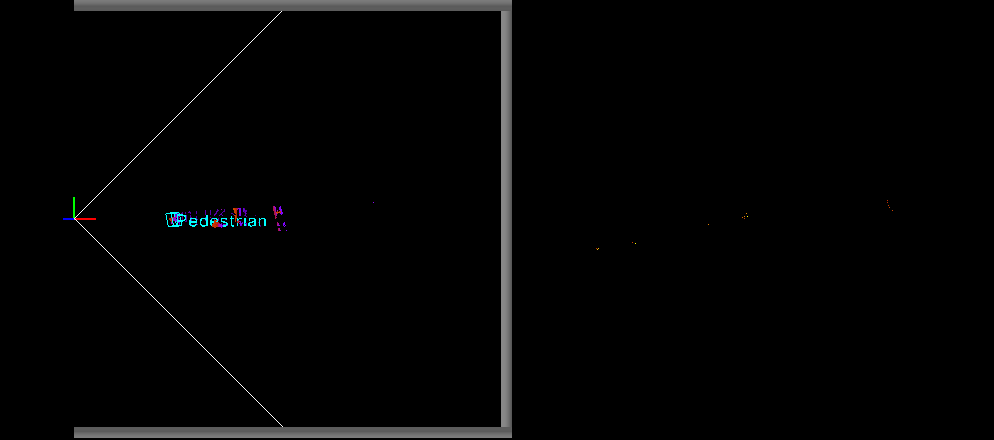
\includegraphics[width=1\linewidth]{Book/figures/7_roi/kitti_pcl_rot_0.png}
	\end{minipage}\hfill
	\begin{minipage}{0.495\textwidth}
		\centering
		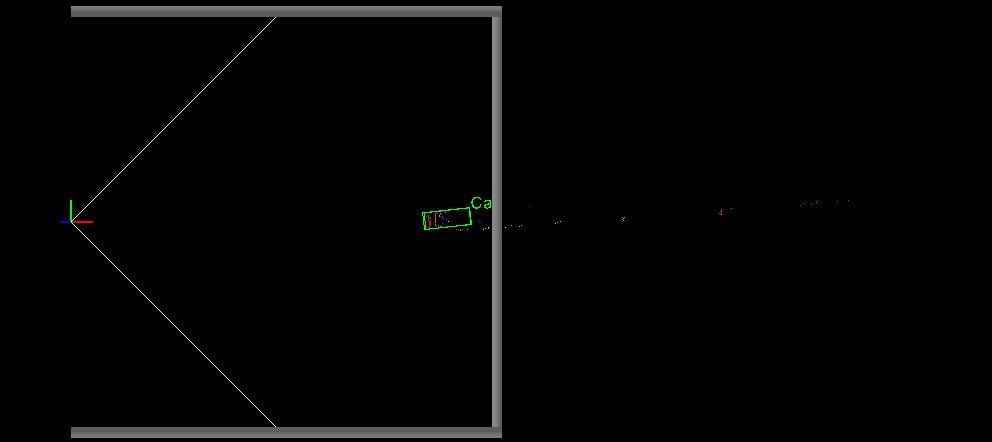
\includegraphics[width=1\linewidth]{Book/figures/7_roi/kitti_pcl_rot_2.png}
	\end{minipage}
	\caption{Nubes de puntos de KITTI rotadas al eje X.}
	\label{fig:Nubes de puntos de KITTI rotadas al eje X.}
\end{figure}

\begin{figure}[H]
	\begin{minipage}{0.495\textwidth}
		\centering
		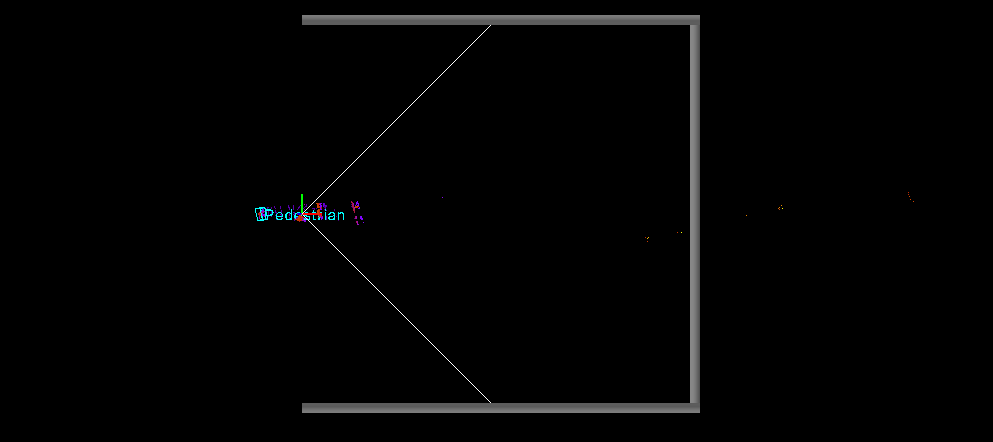
\includegraphics[width=1\linewidth]{Book/figures/7_roi/kitti_pcl_mov_0.png}
	\end{minipage}\hfill
	\begin{minipage}{0.495\textwidth}
		\centering
		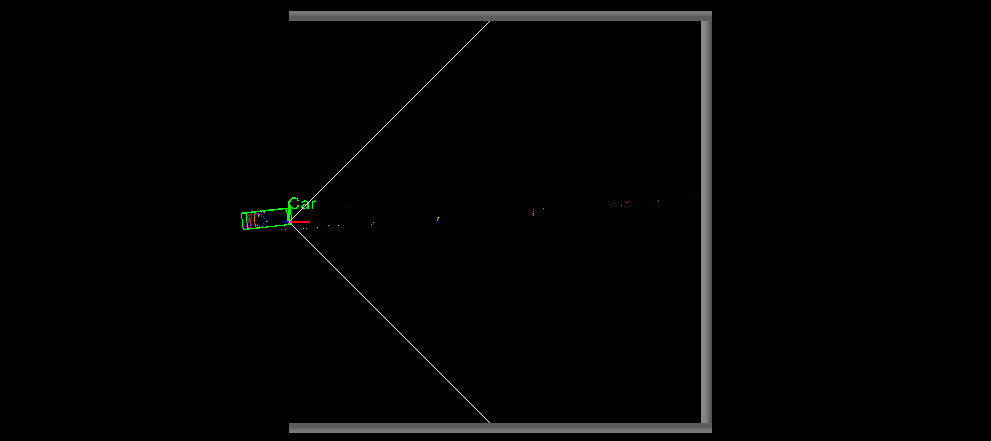
\includegraphics[width=1\linewidth]{Book/figures/7_roi/kitti_pcl_mov_2.png}
	\end{minipage}
	\caption{Nubes de puntos de KITTI movidas al origen de coordenadas.}
	\label{fig:Nubes de puntos de KITTI movidas al origen de coordenadas.}
\end{figure}

\begin{figure}[H]
	\begin{minipage}{0.495\textwidth}
		\centering
		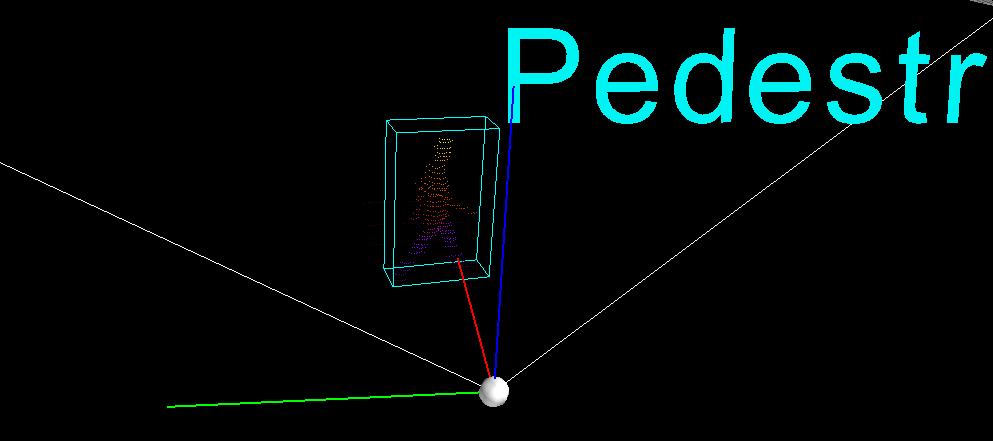
\includegraphics[width=1\linewidth]{Book/figures/7_roi/kitti_pcl_frustum_0.png}
	\end{minipage}\hfill
	\begin{minipage}{0.495\textwidth}
		\centering
		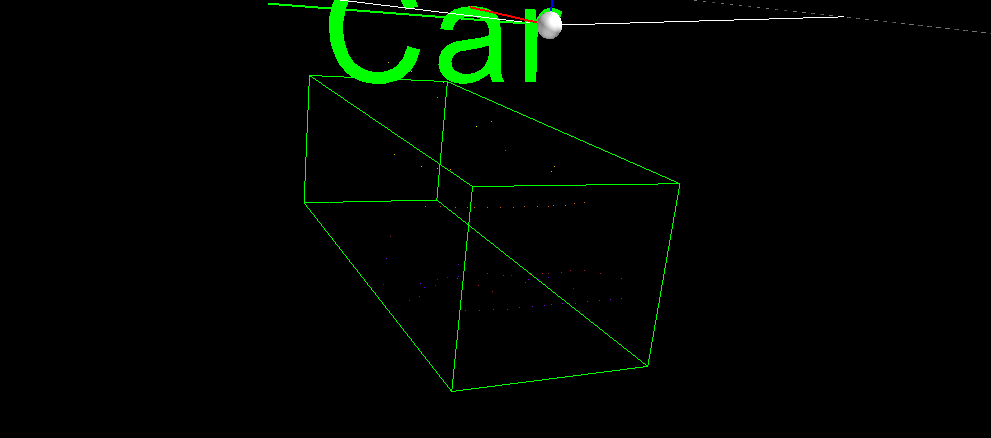
\includegraphics[width=1\linewidth]{Book/figures/7_roi/kitti_pcl_frustum_2.png}
	\end{minipage}
	\caption{Frustums obtenidos a partir de las nubes de puntos de KITTI.}
	\label{fig:Frustums obtenidos a partir de las nubes de puntos de KITTI.}
\end{figure}